% !TeX program = xelatex

\documentclass[landscape,twocolumn,a5paper]{manual}
\usepackage[margin=0.33in,bottom=0.5in,footskip=0.25in]{geometry}

\usepackage{tikz}
\usetikzlibrary{positioning,shapes,backgrounds}
\usepackage{tkz-euclide}

\definecolor{themered}{HTML}{8B3232}
\colorlet{theme}{themered}

\pluginname{ChowTape}

\def\pluginfolder{\href{https://help.uaudio.com/hc/en-us/articles/210216306-Default-Install-Locations-for-UAD-Plug-Ins}{plugin folder}}
\def\dllink#1{\href{https://github.com/jatinchowdhury18/AnalogTapeModel/releases}{#1}}

\begin{document}

\section{ChowTape User Manual}

\noindent
\boldtheme{ChowTape} is an analog tape machine physical model,
originally based on the Sony TC-260. The current version
can be used to emulate a wide variety of reel-to-reel tape
machines, using physics-based emulation algorithms\footnote{The
plugin is based off a 2019 DAFx paper \href{http://dafx2019.bcu.ac.uk/papers/DAFx2019_paper_3.pdf}{``Real-time Physical Modelling for Analog Tape Machines''}.}.
The plugin is currently available for Windows, Linux, Mac, and iOS
in the following formats: VST/VST3, AU, CLAP, LV2,
AAX, AUv3, and Standalone.

\subsection{Installation}
To install ChowTape for desktop, download the plugin installer
from the \href{https://chowdsp.com/products.html#tape}{ChowDSP website}.
If you would like to try the latest changes (unstable), you can
download the latest \href{https://chowdsp.com/nightly.html}{Nightly build}.
It is also possible to compile the plugin
\href{https://github.com/jatinchowdhury18/AnalogTapeModel/blob/master/BUILDING.md}{from the source code}.
ChowTape for iOS can be downloaded from the
\href{https://apps.apple.com/us/app/chowtapemodel/id1557806564}{App Store}.

\begin{figure}[ht]
    \center
    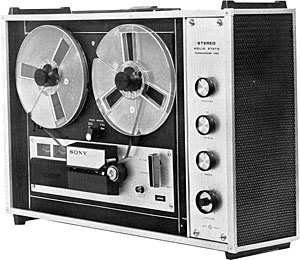
\includegraphics[width=0.45\columnwidth]{sony_tc-260.jpg}
    \caption{\label{TapeMachine}{\it A Sony TC 260 reel-to-reel tape machine}}
\end{figure}

\begin{figure}[ht]
    \center
    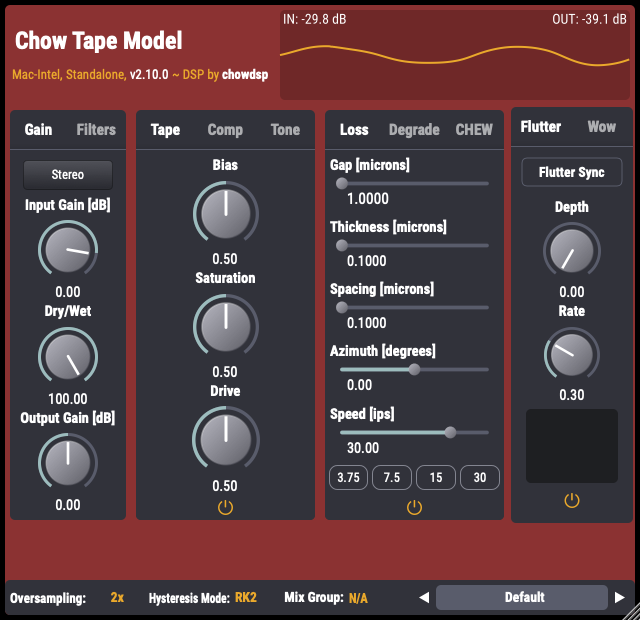
\includegraphics[width=0.55\columnwidth]{../Plugin/Screenshots/full_gui.png}
    \caption{\label{full_gui}{\it ChowTape User Interface}}
\end{figure}

\subsection{Controls}
ChowTape contains a wide range of controls allowing the
user to design the the physical characteristics of the tape
machine and magnetic tape being emulated. Several of the
controls even allow the user to achieve more ``extreme''
results than would be possible with a physical tape machine.
%
%
\begin{figure*}
    \centering
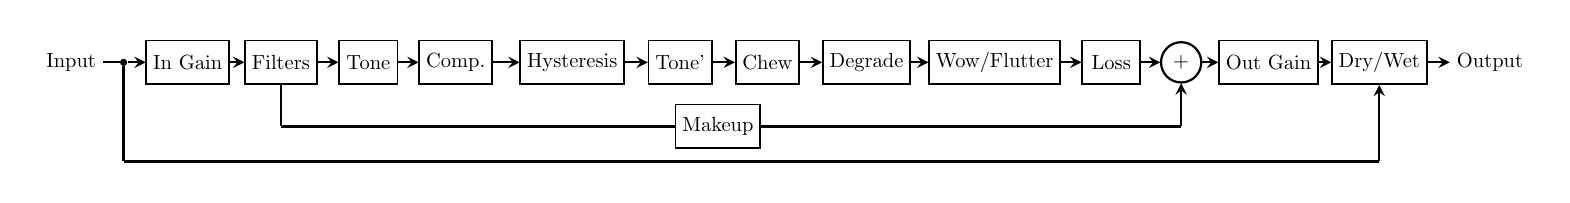
\begin{tikzpicture}[node distance=1.5cm, background rectangle/.style={fill=white}, show background rectangle, every node/.style={scale=0.74}]
    \tikzset{
        mynode/.style = {rectangle, line width=0.65pt, minimum width=1.0cm, minimum height=0.75cm, text centered, draw=black, fill=white},
        arrow/.style = {thick,->,>=stealth},
    }
    \node (input) [xshift=-5.0cm] {Input};
    \node (in_split) [circle, fill, inner sep=1.25pt, right of=input, xshift=-0.6cm] {};
    \node (in_gain) [mynode, right of=in_split, xshift=-0.4cm] {In Gain};
    \node (in_filters) [mynode, right of=in_gain, xshift=0.1cm] {Filters};
    \node (in_tone) [mynode, right of=in_filters, xshift=0.0cm] {Tone};
    \node (comp) [mynode, right of=in_tone, xshift=0.0cm] {Comp.};
    \node (hyst) [mynode, right of=comp, xshift=0.5cm] {Hysteresis};
    \node (out_tone) [mynode, right of=hyst, xshift=0.35cm] {Tone'};
    \node (chew) [mynode, right of=out_tone, xshift=0.0cm] {Chew};
    \node (degrade) [mynode, right of=chew, xshift=0.2cm] {Degrade};
    \node (wow_flutter) [mynode, right of=degrade, xshift=0.7cm] {Wow/Flutter};
    \node (loss) [mynode, right of=wow_flutter, xshift=0.5cm] {Loss};
    \node (sum) [draw, fill=white, circle, line width=0.8pt, right of=loss, xshift=-0.3cm] {+};
    \node (out_gain) [mynode, right of=sum, xshift=0.0cm] {Out Gain};
    \node (dry_wet) [mynode, right of=out_gain, xshift=0.4cm] {Dry/Wet};
    \node (output) [right of=dry_wet, xshift=0.4cm] {Output};

    \draw [thick] (input) -- (in_split);
    \draw [arrow] (in_split) -- (in_gain);
    \draw [arrow] (in_gain) -- (in_filters);
    \draw [arrow] (in_filters) -- (in_tone);
    \draw [arrow] (in_tone) -- (comp);
    \draw [arrow] (comp) -- (hyst);
    \draw [arrow] (hyst) -- (out_tone);
    \draw [arrow] (out_tone) -- (chew);
    \draw [arrow] (chew) -- (degrade);
    \draw [arrow] (degrade) -- (wow_flutter);
    \draw [arrow] (wow_flutter) -- (loss);
    \draw [arrow] (loss) -- (sum);
    \draw [arrow] (sum) -- (out_gain);
    \draw [arrow] (out_gain) -- (dry_wet);
    \draw [arrow] (dry_wet) -- (output);
    
    \coordinate[below of=in_split, yshift=-0.2cm] (down1);
    \coordinate[below of=dry_wet, yshift=-0.2cm] (up1);
    \draw [thick] (in_split) -- (down1);
    \draw [thick] (down1) -- (up1);
    \draw [arrow] (up1) -- (dry_wet);
    
    \coordinate[below of=in_filters, yshift=0.4cm] (down2);
    \coordinate[below of=sum, yshift=0.4cm] (up2);
    \node (makeup) [mynode, right of=down2, xshift=6.0cm] {Makeup};
    \draw [thick] (in_filters) -- (down2);
    \draw [thick] (down2) -- (makeup);
    \draw [thick] (makeup) -- (up2);
    \draw [arrow] (up2) -- (sum);
\end{tikzpicture}
    \caption{\label{fig:tape_dsp}{\it Signal flow for the ChowTape plugin.
                                  Note that the Tone block contains a set
                                  of pre-emphasis filters, while the Tone'
                                  block contains the corresponding post-emphasis
                                  filters.}}
\end{figure*}

\subsubsection{Main Controls}
\boldtheme{Input Gain} controls the gain level going into
the rest of the plugin. Note that abnormally large levels
can cause the plugin to become unstable, so it is recommended
that sound levels are at or below unity gain going into the
plugin, and any extra gain should come from the input gain
control.
\newpar
\boldtheme{Dry/Wet} allows the user to choose how much of the
signal they want to the plugin's processing to affect.
\newpar
\boldtheme{Output Gain} controls the level coming out of the plugin.
\newpar
\boldtheme{Oversampling} controls the amount of oversampling
being done internally within the plugin. More oversampling
will result in a higher quality sound with fewer aliasing
artifacts and better noise characteristics, but will also
use more CPU. It is recommended to use as much oversampling
as your CPU will allow.
\newpar
\boldtheme{Mix Group}: When using ChowTape on multiple channels
in a mix, you can synchronize parameters between plugin
instances belonging to the same mix group. Essentially, all
the plugin instances in the same mix group will share the same
parameters.

\begin{figure}[ht]
    \center
    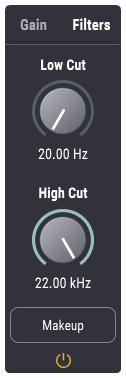
\includegraphics[height=0.32\paperheight]{../Plugin/Screenshots/Filters.png}
    \caption{\label{h_inputs}{\it Input filter controls}}
\end{figure}

\subsubsection{Input Filter Controls}
The ChowTape input filters apply a low-cut and high-cut filter
to the input signal before it is passed on to the rest of the
plugin. The \boldtheme{Low Cut} and \boldtheme{High Cut} knobs
control the cutoff frequencies of the two filters. The
\boldtheme{Makeup} control allows the signal cut out by the
input filters to be added back to the output of the plugin.
Makeup be useful by allowing sub-bass frequencies to pass
through the plugin unaffected.

\begin{figure}[ht]
    \center
    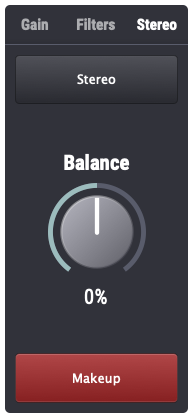
\includegraphics[height=0.32\paperheight]{../Plugin/Screenshots/Stereo.png}
    \caption{\label{h_inputs}{\it Stereo controls}}
\end{figure}

\subsection{Stereo Controls}

When using ChowTape in \boldtheme{Stereo} mode, the plugin
will process the input signal as a left/right pair. In \boldtheme{Mid/Side}
mode, the plugin will encode the input signal as a mid/side pair,
process the mid/side signal, and then decode the signal back to a
left/right stereo pair at the output.
\newpar
The \boldtheme{Balance} control
makes one of the channels louder than the other, either ``panning'' the
signal, or emphasizing either the mid or side part of the signal. The
\boldtheme{Makeup} control allows the signal which was attenuated by
the Balance control to be amplified by the same amount at the output
of the plugin. Makeup can be useful by allowing either the mid or side
part of the signal to be distorted more heavily by the plugin.
When using the plugin with a channel configuration other than stereo,
these controls will have no effect.

\begin{figure}[ht]
    \center
    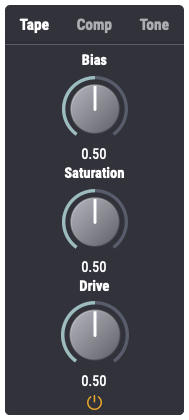
\includegraphics[height=0.4\paperheight]{../Plugin/Screenshots/Tape.png}
    \caption{\label{hysteresis_controls}{\it Tape hysteresis controls}}
\end{figure}
%
% \begin{figure}[ht]
%     \center
%     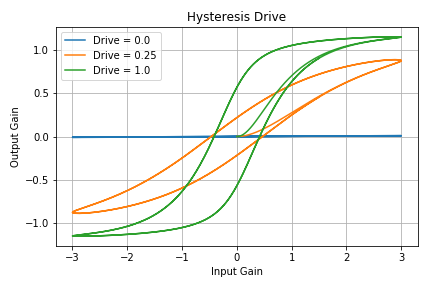
\includegraphics[width=0.9\columnwidth]{../Simulations/Hysteresis/drive.png}
%     \caption{\label{h_drive}{\it Hysteresis curves with varying drive}}
% \end{figure}
%
\begin{figure}[ht]
    \center
    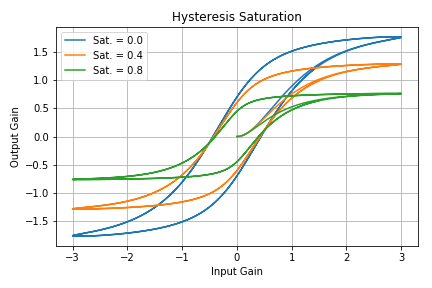
\includegraphics[width=0.85\columnwidth]{../Simulations/Hysteresis/sat.png}
    \caption{\label{h_sat}{\it Hysteresis curves with varying saturation}}
\end{figure}
%
\begin{figure}[]
    \center
    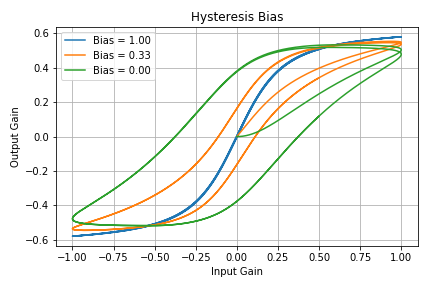
\includegraphics[width=0.85\columnwidth]{../Simulations/Hysteresis/bias.png}
    \caption{\label{h_bias}{\it Hysteresis curves with varying bias}}
\end{figure}

\subsubsection{Hysteresis Controls}
The hysteresis processing is the most important section of the
plugin. \href{https://en.wikipedia.org/wiki/Hysteresis}{Hysteresis}
is a complex nonlinear phenomenon that describes many
natural processes in physics, biology, economics, and more.
In particular, magnetic hysteresis describes the process by
which tape becomes magnetised when subjected to a strong magnetic
field. ChowTape emulates magnetic hysteresis, using the
Jiles-Atherton\footnote{Jiles, D.C.; Atherton, D.L. (1984) ``Theory of ferromagnetic hysteresis'' \textit{Journal of Applied Physics}.}
model of magnetic hysteresis. Magnetic hysteresis is largely
responsible for the ``warm'' sound often associated with
analog tape distortion.
\newpar
\boldtheme{Drive} controls the level of amplification done by
the hysteresis process. This differs from the input gain in that
it affects the nonlinear characteristic of the hysteresis process.
\newpar
\boldtheme{Saturation} controls the level at which the hysteresis
function saturates. Higher values correspond to a lower saturation
point, resulting in a more distorted sound.
\newpar
\boldtheme{Bias} controls the amount of bias used by the tape
recorder. Tape bias is the addition of an inaudible high-frequency
signal to the audio signal\footnote{\href{https://hccc.org.uk/acbias.html}{More information on tape biasing}}.
At lower bias levels, the hysteresis curve becomes ``wider'',
thus creating the ``deadzone'' effect often associated with
underbiased tape.
\newpar
\boldtheme{Hysteresis Mode} selects the equation solver used
to solve the Jiles-Atherton equation in real time. ChowTape
currently supports the following hysteresis modes:
\renewcommand{\labelitemi}{\textendash}
\begin{itemize}
    \itemsep-1mm
    \item 2nd-order Runge Kutta (RK2)
    \item 4th-order Runge Kutta (RK4)
    \item 4-iteration Newton Raphson (NR4)
    \item 8-iteration Newton Raphson (NR8)
    \item State Transition Network\footnote{Parker, J.D. et. al. (2019) ``Modelling of Nonlinear State-Space Systems using a Deep Neural Network'' \textit{Proc. 22\textsuperscript{nd} Int. Conference on Digital Audio Effects}.} (STN)
    \item Version 1.0 processing (V1)
\end{itemize}
%
The Runge-Kutta solvers are computationally cheaper, but
somewhat less accurate than the Newton-Raphson solvers.
Similarly, the higher-order solvers will be more accurate,
but will also consume more compute resources. The State
Transition Network is designed to be a computationally
cheaper approximation of the NR8 solver; although it
distorts more harshly at extreme settings. The V1 mode
reverts to a different parameterization of the hysteresis
equation that was used in earlier versions of the plugin. It
is recommended to use higher-order solvers for mix busses
and key tracks in a mix, while using lower-order solvers for
less important tracks.

\begin{figure}[ht]
    \center
    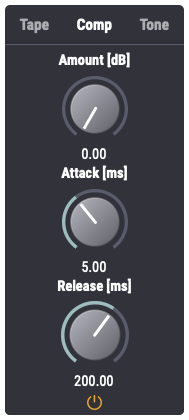
\includegraphics[height=0.35\paperheight]{../Plugin/Screenshots/Comp.png}
    \caption{\label{comp_controls}{\it Tape compression controls}}
\end{figure}
%
\subsubsection{Compression Controls}
The compression section applies a characteristic
compression curve to the signal, which can be useful
for reducing the dynamic range of the signal before
going into the hysteresis processing.
\newpar
\boldtheme{Amount} controls the level at which the
compression curve starts to take effect. At 0 dB, the
compression has no effect on the signal. At 9 dB, any
signal above -9 dB will start to be compressed.
\newpar
The \boldtheme{Attack} parameter controls how quickly
the compression will start to take effect once the
signal enters the range where it is being compressed.
\newpar
Similarly, the \boldtheme{Release} parameter controls
how quickly the compression backs off once the signal
is no longer in the compression region.
%
\begin{figure}[ht]
    \center
    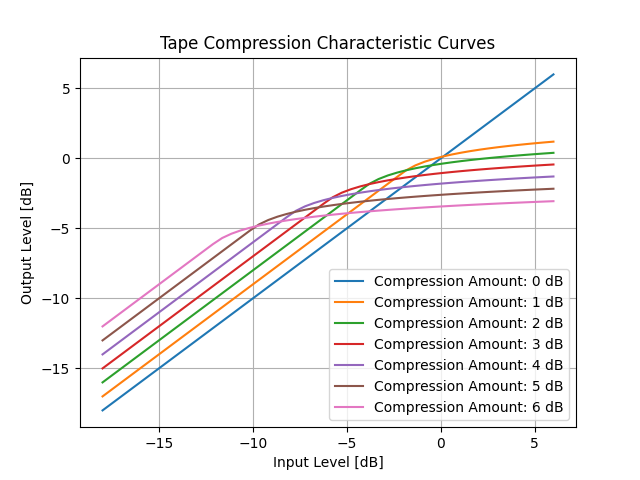
\includegraphics[width=0.9\columnwidth]{../Simulations/Compression/compression_curves.png}
    \caption{\label{comp_curves}{\it Tape compression characteristic curves}}
\end{figure}

\subsubsection{Tone Controls}
The tone section applies a set of pre-/post-emphasis filters
to the signal before and after the hysteresis processing
is applied. The filters work similar to
\href{https://en.wikipedia.org/wiki/RIAA_equalization}{RIAA filters},
in that the pre- and post- filters have exact opposite frequency
responses.
\newpar
The \boldtheme{Bass} and \boldtheme{Treble} knobs control
the frequency response of the pre-emphasis filter, and the
post-emphasis filter will automatically adjust. The
\boldtheme{Frequency} knob controls the transition frequency
between the bass and treble sections of the filter.

\begin{figure}[ht]
    \center
    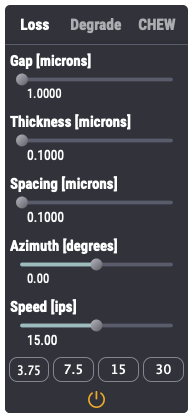
\includegraphics[height=0.45\paperheight]{../Plugin/Screenshots/Loss.png}
    \caption{\label{loss_controls}{\it Loss filter controls}}
\end{figure}
%
\begin{figure}[ht]
    \center
    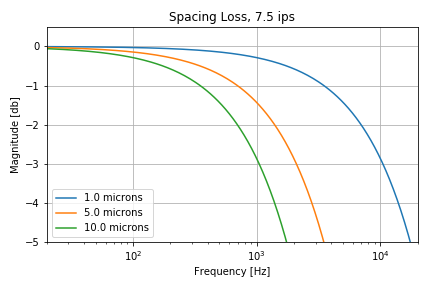
\includegraphics[width=0.85\columnwidth]{../Simulations/LossEffects/space_loss.png}
    \caption{\label{spacing_loss}{\it Spacing loss at 7.5 ips}}
\end{figure}
%
\begin{figure}[ht]
    \center
    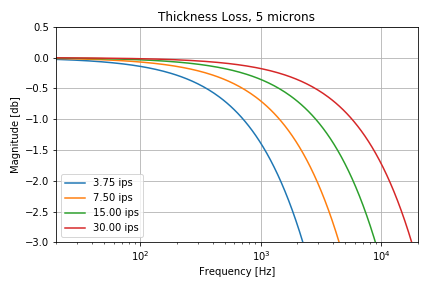
\includegraphics[width=0.85\columnwidth]{../Simulations/LossEffects/speed_thickness.png}
    \caption{\label{thick_loss}{\it Thickness loss for 5 micron tape}}
\end{figure}

\subsubsection{Playhead Controls}
Physical tape machines also have a frequency response that
is affected by the amount of space between the playhead and
the tape, the width of the playhead gap, and the thickness
of tape used. The frequency responses of each of these ``loss
effects'' is also dependent on the tape speed.
\newpar
\boldtheme{Spacing}
controls the amount of space between the playhead and the tape,
measured in centimeters.
\newpar
\boldtheme{Thickness} controls the thickness
of the tape, measured in centimeters.
\newpar
\boldtheme{Gap} controls
the width of the playhead gap, measured in millimeters.
\newpar
\boldtheme{Azimuth}
controls the playhead alignment angle\footnote{\href{https://blog.weareavp.com/azimuth-adjustment-for-magnetic-audio-recordings}{More information on playhead azimuth}.}.
A misalignment between the playhead and the tape causes a
corresponding time misalignment between the two stereo tracks
on the tape, resulting in a stereo ``widening'' effect.
\newpar
\boldtheme{Speed}
controls the tape speed as it effects the above loss effects,
measured in inches per second (ips). While this control is
continuous, the parameter can be quantized to the standard speeds
for reel-to-reel tape machines: 3.75, 7.5, 15, and 30 ips.
\newline
\newline
\newline
\subsubsection{Tape Degradation Controls}
The degradatation parameters control a simulation of
old tape that has been used over and over, and has started
to degrade.
\newline
\boldtheme{Depth}
controls the intensity of the wear on the tape. Enable the
\boldtheme{0.1x} option to make this control more subtle.
\newpar
\boldtheme{Amount}
controls the amount of wear, typically corresponding to
the age of the tape.
\newpar
\boldtheme{Variance}
adds a time-varying randomness to the degradatation.
\newpar
\boldtheme{Envelope}
applies an amplitude envelope to the tape noise.

\begin{figure}[ht]
    \center
    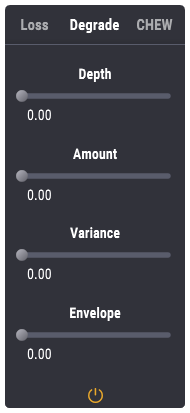
\includegraphics[height=0.4\paperheight]{../Plugin/Screenshots/Degrade.png}
    \caption{\label{degrade_controls}{\it Degradation controls.}}
\end{figure}

\subsubsection{Chew Controls}
The chew parameters simulate tape that has been chewed up by
a broken tape machine. \boldtheme{Depth} controls how deep the
tape is chewed, \boldtheme{Frequency} controls how much space
there is between bits of tape that have been chewed up, and
\boldtheme{Variance} determines how much randomness there is
in determining the amount of space between chewed up sections.

\subsubsection{Wow and Flutter Controls}
Tape machines also exhibit timing irregularities, often due
to small imperfections in the mechanics of the machine causing
the tape to subtly speed up and slow down while being
played back. The flutter characteristic in this plugin was
captured from an original Sony TC-260 tape machine.
%
\begin{figure}[ht]
    \center
    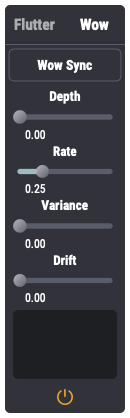
\includegraphics[height=0.35\paperheight]{../Plugin/Screenshots/Wow.png}
    \caption{\label{wow_controls}{\it Wow controls.}}
\end{figure}
%
\newline
\boldtheme{Depth} controls the depth of the flutter and
\boldtheme{Rate} controls the rate of flutter, with higher values
causing the flutter to occur faster. Note that the
flutter rate can be synchronized to the tape speed, or to the
tempo of the song.
\newpar
"\boldtheme{Wow}" is similar to flutter but on a much longer time scale,
and contains similar controls, as well as \boldtheme{Variance} and
\boldtheme{Drift} which control the random irregularities that
cause the wow characteristic.

\subsection{Presets}
Presets provide a quick way to achieve a specific sound
with the plugin. ChowTape comes with a set of built-in
factory presets. To contribute your presets to be added
to the factory presets list for future releases, see the
\href{https://github.com/jatinchowdhury18/AnalogTapeModel/issues/30}{Presets GitHub issue}.

\subsubsection{User Presets}
To save the current plugin state as a user preset, open
the presets menu, and select ``Save''. The first time a
preset is saved, you will be asked to choose a preset
folder. All future presets will be saved to this folder,
and when the plugin opens, it will search this folder, as
well as any subfolders, to load new user presets.
Presets located in subfolders will be placed in their
own groups in the preset menu.
\newline

\subsection{Accessibility}
ChowTape includes accessibility for screen readers on Windows
and Mac OS. All the controls in the user interface may be navigated
using either the screen reader's navigation keys, or using the ``Tab''
key. Users may interact with buttons and menus using the ``Enter'' key.
For continuous slider controls, the following keyboard shortcuts are
supported:
\renewcommand{\labelitemi}{\textendash}
\begin{itemize}
    \itemsep-1mm
    \item Up/Down Arrow Key: Nudge the slider value.
    \item Page-Up/Page-Down Key: ``Big'' nudge the slider value.
    \item Delete Key: Move the slider to its default value.
    \item Home Key: Move the slider to its minimum value.
    \item End Key: Move the slider to its maximum value.
\end{itemize}
%
Note that Windows users will want to ensure that OpenGL is turned off
when using the plugin with a screen reader, otherwise the screen reader
software may not be able to navigate into the plugin window.

\subsection{Troubleshooting}
If you run into issues when using ChowTape, you may submit bug reports
using GitHub Issues. However, it is recommended to read the following
troubleshooting suggestions first.

\subsubsection{Resetting Global Settings}
If you run into any issues that require the global settings to
be changed or reset, the global settings file can be found in the
users ``AppData'' directory (Windows), ``Library'' directory (Mac OS),
or ``.config'' directory (Linux). To reset the global settings, you may
delete this file, and it will automatically be regenerated the next time
the plugin is used.

\subsubsection{OpenGL Rendering}
On Windows and Linux, ChowTape will have the option to use OpenGL
for rendering the UI, unless the host system does not support OpenGL
version 2.0 or greater. If OpenGL is available, it is possible to turn
rendering with OpenGL on or off in the global settings menu. If you
need to override your chosen OpenGL setting, please visit the global
settings file.

\subsubsection{Copying Plugin Diagnostics}
If you need to submit a bug report, it is very useful to include
the plugin's diagnostic information in your bug report. The diagnostic
info can be copied from the global settings menu.

\subsection{Open Source}
ChowTape is open-source software that is free (as in ``free
beer''), and free (as in ``free speech''), under the
\href{https://www.gnu.org/licenses/gpl-3.0}{General Public License}.
As a research project, the goal of developing this plugin is
to help advance the body of knowledge of real-time audio
signal processing. Therefore, keeping any part of this project
behind a paywall, or licensing this software under a proprietary
license would be antithetical to that goal. As an open-source
project, ChowTape is open to outside contributors. For more
information, see our
\href{https://github.com/jatinchowdhury18/AnalogTapeModel/blob/master/CONTRIBUTING.md}{Contributing}
page.

\subsection{Feedback}
If you notice any bugs, or have any questions, feel free
to \href{mailto:chowdsp@gmail.com}{email me directly},
or \href{https://github.com/jatinchowdhury18/AnalogTapeModel/issues}{create an issue ticket}
on GitHub. GitHub issues are preferred, since they are publicly
visible.

\subsection{Acknowledgements}
Thanks to Yann from SINK Music for helping to create this
user manual, as well as all the users of ChowTape who have
made efforts to help improve the plugin.
\newpar
Enjoy!
\newpar
Jatin Chowdhury
\newpar
\href{https://github.com/jatinchowdhury18/AnalogTapeModel}{https://github.com/jatinchowdhury18/AnalogTapeModel}

\end{document}
